% GENERATED by make_paper_assets.py -- do not edit by hand.
\begin{figure}[t]
\centering
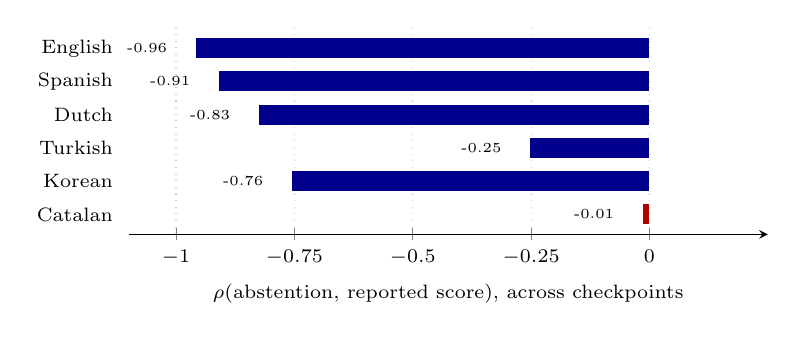
\begin{tikzpicture}
\begin{axis}[
  width=0.80\columnwidth, height=4.2cm, xmin=-1.1, xmax=0.25, ymin=0.4, ymax=6.6,
  xtick={-1,-0.75,-0.5,-0.25,0},
  ytick={6,5,4,3,2,1}, yticklabels={English,Spanish,Dutch,Turkish,Korean,Catalan},
  xlabel={$\rho$(abstention, reported score), across checkpoints},
  tick label style={font=\scriptsize}, label style={font=\scriptsize},
  axis lines=left, y axis line style={draw=none}, ytick style={draw=none},
  xmajorgrids, grid style={dotted, gray!40}, clip=false,
]
\fill[blue!55!black] (axis cs:0,5.7) rectangle (axis cs:-0.958,6.3);
\node[font=\tiny, anchor=east] at (axis cs:-0.998,6) {-0.96};
\fill[blue!55!black] (axis cs:0,4.7) rectangle (axis cs:-0.909,5.3);
\node[font=\tiny, anchor=east] at (axis cs:-0.949,5) {-0.91};
\fill[blue!55!black] (axis cs:0,3.7) rectangle (axis cs:-0.825,4.3);
\node[font=\tiny, anchor=east] at (axis cs:-0.865,4) {-0.83};
\fill[blue!55!black] (axis cs:0,2.7) rectangle (axis cs:-0.252,3.3);
\node[font=\tiny, anchor=east] at (axis cs:-0.292,3) {-0.25};
\fill[blue!55!black] (axis cs:0,1.7) rectangle (axis cs:-0.755,2.3);
\node[font=\tiny, anchor=east] at (axis cs:-0.795,2) {-0.76};
\fill[red!70!black] (axis cs:0,0.7) rectangle (axis cs:-0.014,1.3);
\node[font=\tiny, anchor=east] at (axis cs:-0.054,1) {-0.01};
\end{axis}
\end{tikzpicture}
\caption{The between-checkpoint correlation behind Table~\ref{tab:multilingual},
by language. Strongly negative in five of six, consistent with abstention
mechanically driving the reported score. Catalan (red) is the exception:
committed-answer bias collapses for four of twelve checkpoints there
(Figure~\ref{fig:catalan-mechanism}), breaking the near-uniform bias the
correlation otherwise relies on.}
\label{fig:multilingual-rho}
\end{figure}
